%!TEX TS-program = xelatex
%!TEX encoding = UTF-8 Unicode
%!TEX root = 2022-GS-ARTICLE.tex
%----------------------------------------------------------------- LANGUAGES ---
\newcommand{\mylanguages}{italian,english} % in reverse order
%---------------------------------------------------------- TITLE & SUBTITLE ---
\newcommand{\mytitle}{General Relativity}
\newcommand{\mysubtitle}{For a more accessible and less technical introduction
                         to this topic, \\ see Introduction to General Relativity}
%----------------------------------------------------------------- AUTHOR(s) ---
\newcommand{\authorone}{Orgo Wikipedio}
\newcommand{\institutione}{Conservatorio S. Cecilia di Roma}
\newcommand{\emailone}{orgo @ wikipedio.com}
%-------------------------------------------------------------------------------
% \newcommand{\authortwo}{Wikio Orgopedio}
% \newcommand{\institutiontwo}{Conservatorio S. Cecilia di Roma}
% \newcommand{\emailtwo}{wikio @ orgopedio.com} % duplicate these 3 lines if more
%-------------------------------------------------------------- STYLE GS2020 ---
%!TEX TS-program = xelatex
%!TEX encoding = UTF-8 Unicode
%!TEX root = 2022-GS-ARTICLE.tex
%-------------------------------- PACKAGES AND OTHER DOCUMENT CONFIGURATIONS ---
\documentclass[
	a4paper,
	twocolumn,
	twoside,
	%openright
]{article}
\usepackage[
	top=20mm,
	bottom=25mm,
	textwidth=17.2cm,
	columnsep=0.8cm,
	bindingoffset=1cm,
	showframe
]{geometry}
\usepackage[T1]{fontenc}
\usepackage[\mylanguages]{babel}
\usepackage{csquotes}
%\usepackage{parskip}
\usepackage[style=authoryear-ibid,backend=biber]{biblatex}
\bibliography{includes/bibliography.bib}
\usepackage{dblfloatfix}
\usepackage{subfigure}
\usepackage[subfigure]{tocloft}
\advance\cftsecnumwidth 0.5em\relax
\advance\cftsubsecindent 0.5em\relax
\advance\cftsubsecnumwidth 0.5em\relax
\usepackage{graphicx}
\usepackage{wrapfig}
% \usepackage{epstopdf}
% \epstopdfsetup{update}
\usepackage[usenames]{color}
\usepackage{xcolor}
\usepackage{tikz}
\usetikzlibrary{shapes,
                through,
								calc,
								intersections,
								backgrounds,
                positioning}
\usepackage{tkz-euclide}
\usepackage{amssymb}
\usepackage[
  colorlinks=true,
  linkcolor=black,
	anchorcolor=black,
	citecolor=black,
	filecolor=black,
	menucolor=black,
	runcolor=black,
	urlcolor=black
	]{hyperref}
\usepackage{Alegreya}
\linespread{1.05}
\usepackage{
	fontspec,
	xltxtra,
	xunicode
	}
\usepackage{
	xfrac,
	unicode-math
	}

\defaultfontfeatures{Mapping=tex-text}
\setmonofont[
	Scale=MatchLowercase
	]{Andale Mono}
\setmathfont[
	Scale=MatchLowercase,
	Scale=1
	]{Libertinus Math}

\usepackage{microtype}

\usepackage[
	hang,
	small,
	labelfont=bf,
	up,
	textfont=it,
	up
	]{caption}
\usepackage{paralist} % For compact item lists
\usepackage{etoolbox} % Some tools: used for quote environment
\AtBeginEnvironment{quote}{\small}
\usepackage{titling} % Customizing the title section
\usepackage{booktabs} % Horizontal rules in tables
\usepackage{enumitem} % Customized lists
\setlist[itemize]{noitemsep} % Make itemize lists more compact
\usepackage{abstract} % Allows abstract customization
\renewcommand{\abstractnamefont}{\normalfont\bfseries} % Set the "Abstract" text to bold
\renewcommand{\abstracttextfont}{\normalfont\small\itshape} % Set the abstract itself to small italic text
\usepackage{titlesec} % Allows customization of titles
\renewcommand\thesection{\Roman{section}} % Roman numerals for the sections
\renewcommand\thesubsection{\Roman{subsection}} % roman numerals for subsections
\titleformat{\section}[block]{\Large}{\thesection.}{1em}{} % Change the look of the section titles
\titleformat{\subsection}[block]{\large}{\thesubsection.}{1em}{} % Change the look of the section titles
%------------------------------------------------------------- TITLE SECTION ---
\setlength{\droptitle}{-4\baselineskip} % Move the title up
\pretitle{\begin{center}\huge\bfseries} % Article title formatting
\posttitle{\end{center}} % Article title closing formatting
\title{\mytitle \\[0.1cm] \large{\emph{\mysubtitle}}} % Article title
\author{%
\textsc{\authorone}\\%
\normalsize \institutione \\ %
\normalsize \emailone %
% activate
% \and % duplicate these 4 lines if more
% \textsc{\authortwo} \\%
% \normalsize \institutiontwo \\ %
% \normalsize \emailtwo %
}
\date{} % Leave empty to omit a date

\usepackage{fancyhdr} % Headers and footers
\pagestyle{fancy} % All pages have headers and footers
\fancyhead{} % Blank out the default header
\fancyfoot{} % Blank out the default footer
\fancyhead[C]{\small Wikipedia • General Relativity} % Custom header text
\fancyfoot[RO]{\small \today~ • w: \input{includes/words.txt} • c: \input{includes/char.txt} • p:~\thepage} % Custom footer text
\fancyfoot[LE]{\small p:~\thepage~ • c: \input{includes/char.txt} • w: \input{includes/words.txt} • \today} % Custom footer text

%-------------------------------------------------------------------------------
%-------------------------------------------------------------------------------
%	LISTINGS
%-------------------------------------------------------------------------------
%-------------------------------------------------------------------------------
\usepackage{listings}
% lstlistings setup
\definecolor{gsbg}{rgb}{0.98,0.98,0.98}

\lstset{%
  aboveskip=10pt,
	belowskip=5pt,
  language=C++,
  numbers=none,%left,%none,
  tabsize=4,
  %frame=single,
  breaklines=true,
  numberstyle=\tiny\ttfamily,
  backgroundcolor=\color{gsbg},
  basicstyle=\footnotesize\ttfamily,
  %commentstyle=\slshape\color{mylstcmt}, %\itshape,
  %frameround=tttt,
  columns=flexible, %fixed,
  showstringspaces=false,
  emptylines=2,
  inputencoding=utf8,
  extendedchars=true,
  literate=	{á}{{\'a}}1
			{à}{{\`a}}1
			{ä}{{\"a}}1
			{â}{{\^a}}1
			{é}{{\'e}}1
			{è}{{\`e}}1
			{ë}{{\"e}}1
			{ê}{{\^e}}1
			{ï}{{\"i}}1
			{î}{{\^i}}1
			{ö}{{\"o}}1
			{ô}{{\^o}}1
			{è}{{\`e}}1
			{ù}{{\`u}}1
			{û}{{\^u}}1
			{ç}{{\c{c}}}1
			{Ç}{{\c{C}}}1,
  emph={component, declare, environment, import, library, process},
  emph={[2]ffunction, fconstant, fvariable},
  emph={[3]button, checkbox, vslider, hslider, nentry, vgroup, hgroup, tgroup, vbargraph, hbargraph, attach},
  %emphstyle=\color{yotxt}, %\underline, %\bfseries,
  %morecomment=[s][\color{mylstdoc}]{<mdoc>}{</mdoc>},
  rulecolor=\color{black}
}

\usepackage[framemethod=tikz]{mdframed} % Allows defining custom boxed/framed environments

%-------------------------------------------------------------------------------
%--------------------------------------------------- INFORMATION ENVIRONMENT ---
%-------------------------------------------------------------------------------

% Usage:
% \begin{info}[optional title, defaults to "Info:"]
% 	contents
% 	\end{info}

\mdfdefinestyle{info}{%
	topline=false, bottomline=false,
	leftline=false, rightline=false,
	nobreak,
	singleextra={%
		\fill[black](P-|O)circle[radius=0.4em];
		\node at(P-|O){\color{white}\scriptsize\bf i};
		\draw[very thick](P-|O)++(0,-0.8em)--(O);%--(O-|P);
	}
}

% Define a custom environment for information
\newenvironment{info}[1][Info:]{ % Set the default title to "Info:"
	\medskip
	\begin{mdframed}[style=info]
		\footnotesize\noindent{\textbf{#1}}
}{
	\end{mdframed}
}

%-------------------------------------------------------------------------------
%----------------------------------------------------- BIOGRAFIA ENVIRONMENT ---
%-------------------------------------------------------------------------------

% Usage:
% \begin{bio}[optional title, defaults to "Info:"]
% 	contents
% 	\end{bio}

\mdfdefinestyle{bio}{%
	topline=false, bottomline=false,
	leftline=false, rightline=false,
	nobreak,
	singleextra={%
		\fill[black](P-|O)circle[radius=0.4em];
		\node at(P-|O){\color{white}\scriptsize\bf b};
		\draw[very thick](P-|O)++(0,-0.8em)--(O);%--(O-|P);
	}
}

% Define a custom environment for information
\newenvironment{bio}[1][Biografia:]{ % Set the default title to "Info:"
	\medskip
	\begin{mdframed}[style=bio]
		\noindent{\textbf{#1}}
}{
	\end{mdframed}
}

%-------------------------------------------------------------------------------
%------------------------------------------------------- WARNING ENVIRONMENT ---
%-------------------------------------------------------------------------------

% Usage:
% \begin{warn}[optional title, defaults to "Warning:"]
%	Contents
% \end{warn}

\mdfdefinestyle{warning}{
	topline=false, bottomline=false,
	leftline=false, rightline=false,
	nobreak,
	singleextra={%
		\draw(P-|O)++(-0.5em,0)node(tmp1){};
		\draw(P-|O)++(0.5em,0)node(tmp2){};
		\fill[black,rotate around={45:(P-|O)}](tmp1)rectangle(tmp2);
		\node at(P-|O){\color{white}\scriptsize\bf !};
		\draw[very thick](P-|O)++(0,-1em)--(O);%--(O-|P);
	}
}

% Define a custom environment for warning text
\newenvironment{warn}[1][Warning:]{ % Set the default warning to "Warning:"
	\medskip
	\begin{mdframed}[style=warning]
		\noindent{\textbf{#1}}
}{
	\end{mdframed}
}

%-------------------------------------------------------------------- ABSTRACT -
\renewcommand{\maketitlehookd}{%
\begin{abstract}
\noindent\input{includes/abstract.txt}
\end{abstract}
}

%------------------------------------------------------------ BEGIN DOCUMENT ---
\begin{document}
\maketitle
\thispagestyle{empty}
%-------------------------------------------------------------------- ABSTRACT -
% The abstract is an external txt file inside the includes folder
%-------------------------------------------------------------------------------
\section*{Disposizione dei microfoni}
Per la ripresa dell'intera orchestra sono stati utilizzati 10 microfoni omni direzionali di modello OM1 della LineAudio organizzati in coppie stereofoniche.
Il punto di ripresa principale è costituito da un ORTF, ovvero una coppia stereofonica semi spaziata con una distanza di 17cm circa tra le due capsule (circa la stessa distanza che intercorre tra le orecchie in un cranio umano) inclinate di 110° circa che permette di riprendere l'ambiente in maniera tridimensionale, fornendo informazioni relative alla profondità dell'ambiente acustico. In questo caso, L'ORTF è stato posto di fronte all'orchestra in corrispondenza del pianoforte e del direttore d'orchestra, a fronte palco.

\subsection*{ruoli}
Ciascuno dei 10 microfoni omnidirezionali ha un ruolo preciso:
Uno per i primi violini ed uno per le viole, posizionati specularmente nell'orchestra a distanza di 425cm l'uno dll'altro.
Tre per i fiati, dei quali uno centrale e due laterali, per allargarne l'immagine. Per questa sezione sono stati utilizzati tre microfoni per due motivi principali: anzitutto perchè la sezione è molto ampia ovvero 428cm, in secondo luogo per catturare anche i timpani, e in particolar modo il dettaglio, essendo storicamente utilizzati per dare sostegno ai fiati: per dare attacco e corpo al  suono.
Due in configurazione stereo AB LR a distanza di 28cm l'uno dall'altro per il pianoforte per catturarne il dettaglio.
Uno come spot per i contrabbassi,posto a 309cm dal flankR, solo per poter compensare il loro dettaglio che sicuramente manca al resto: la sua utilità si limita a questo, in quanto non potrebbe dare informazioni sulla profondità della sezione trattandosi di un microfono mono, così come non potrebbe riprenderne fedelmente le basse frequenze essendo un microfono di spot e quindi molto vicino alla sorgente, anche perchè le basse frequenze dei contrabbassi così come degli altri strumenti (in particolar modo dei timpani) saranno già riprese fedelmente dai microfoni main, essendo questi molto distanti dalla sorgente.
Due utilizzati come Flanks, ovvero di sostegno all'ORTF a distanza speculare di 324cm per allargarne l'immagine dell'intera orchestra. Il complesso Flanks + ORTF costituisce la ripresa main dell'orchestra, ovvero quella generale, la quale non serve a catturare i singoli dettagli, quanto a dare un'immagine complessiva frontale dell'orchestra.


\section*{Gestione del materiale}

\subsection*{sessione di registrazione}

\subsection*{Mid Side}
Perchè trattare il materiale delle registrazioni in Mid Side? In questa configurazione, è possibile gestire l'ambiente come uno spazio trigonometrico, in quanto la gestione dell'ambiente custico non è solo relativa alle ampiezze delle riflessioni come in configurazione stereo, ma è possibile percepire la profondità di una fonte sonora avendo l'ambiente su un canale separato.



\section*{UNNUMBERED SECTION}
Some predictions of general relativity differ significantly from those of
classical physics, especially concerning the passage of time, the geometry of
space, the motion of bodies in free fall, and the propagation of light. Examples
of such differences include gravitational time dilation, gravitational lensing,
the gravitational redshift of light, and the gravitational time delay. The
predictions of general relativity in relation to classical physics have been
confirmed in all observations and experiments to date. Although general
relativity is not the only relativistic theory of gravity, it is the simplest
theory that is consistent with experimental data. However, unanswered questions
remain, the most fundamental being how general relativity can be reconciled with
the laws of quantum physics to produce a complete and self-consistent theory of
quantum gravity.
%-------------------------------------------------------------------------------
\subsection*{UNNUMBERED SUB-SECTION}

\begin{warn}[Einstein's theory]
 has important astrophysical implications. For example, it
implies the existence of black holes regions of space in which space and time
are distorted in such a way that nothing, not even light, can escape as an
end state for massive stars.
\end{warn}

There is ample evidence that the intense radiation
emitted by certain kinds of astronomical objects is due to black holes. For
example, microquasars and active galactic nuclei result from the presence of
stellar black holes and supermassive black holes, respectively. The bending of
light by gravity can lead to the phenomenon of gravitational lensing, in which
multiple images of the same distant astronomical object are visible in the sky.
General relativity also predicts the existence of gravitational waves, which
have since been observed directly by the physics collaboration LIGO.
%-------------------------------------------------------------------------------
\subsubsection*{UNNUMBERED SUB-SUB-SECTION}
Some predictions of general relativity differ significantly from those of
classical physics, especially concerning the passage of time, the geometry of
space, the motion of bodies in free fall, and the propagation of light. Examples
of such differences include gravitational time dilation, gravitational lensing,
the gravitational redshift of light, and the gravitational time delay. The
predictions of general relativity in relation to classical physics have been
confirmed in all observations and experiments to date. Although general
relativity is not the only relativistic theory of gravity, it is the simplest
theory that is consistent with experimental data. However, unanswered questions
remain, the most fundamental being how general relativity can be reconciled with
the laws of quantum physics to produce a complete and self-consistent theory of
quantum gravity.

Einstein's theory has important astrophysical implications. For example, it
implies the existence of black holes regions of space in which space and time
are distorted in such a way that nothing, not even light, can escape as an
end state for massive stars. There is ample evidence that the intense radiation
emitted by certain kinds of astronomical objects is due to black holes. For
example, microquasars and active galactic nuclei result from the presence of
stellar black holes and supermassive black holes\ldots


\vfill\null

\begin{figure}[b]
\begin{center}
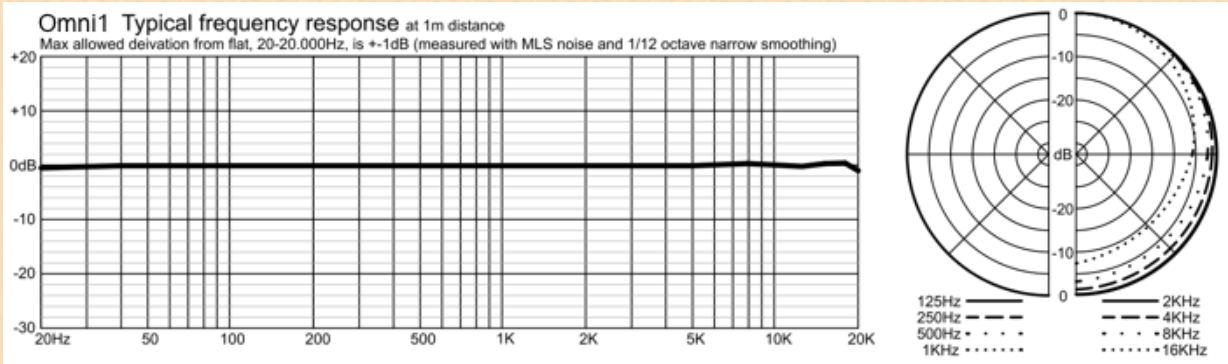
\includegraphics[width=.47\textwidth]{img/image1.png}
\caption{\textbf{Spacetime curvature schematic}. Lattice analogy of the deformation
of spacetime caused by a planetary mass.}
\label{gr01}
\end{center}
\end{figure}

\newpage % USE NEWPAGE TO FORCE COLUMNN INTERRUPTION
%-------------------------------------------------------------------------------
%-------------------------------------------------------------------------------
\section*{UNNUMBERED SECTION}

\begin{quote}
La musica non e` solo composizione. \\
Non è artigianato, non è un mestiere. \\
La musica è pensiero. \cite{nono85}
\end{quote}

Some predictions of general relativity differ significantly from those of
classical physics, especially concerning the passage of time, the geometry of
space, the motion of bodies in free fall, and the propagation of light. Examples
of such differences include gravitational time dilation, gravitational lensing,
the gravitational redshift of light, and the gravitational time delay. The
predictions of general relativity in relation to classical physics have been
confirmed in all observations and experiments to date. Although general
relativity is not the only relativistic theory of gravity, it is the simplest
theory that is consistent with experimental data. However, unanswered questions
remain, the most fundamental being how general relativity can be reconciled with
the laws of quantum physics to produce a complete and self-consistent theory of
quantum gravity.

\begin{table}[htp]
\begin{center}
\begin{tabular}{ll}
\textbf{Stages} & \textbf{Dur.} \\
\hline
\textbf{Omnidirectional Expositions} & 6 mo. \\
Sound-shape analysis and visualizations & \\
Sound-shape reproduction & \\
Sound-shape database design & \\
\hline
\textbf{Micro-Rhythm of sound-shape} & 12 mo. \\
Solo repertoire analysis & \\
Sound-shape explosion in practising & \\
From literature to shapes open-data & \\
\hline
\textbf{Rhythm of sound-shape interactions} & 12 mo. \\
Multiple sources multiple shapes & \\
Relationship and complexity perception & \\
\hline
\textbf{Sound-shape in musical composition} & 12 mo. \\
AI: unleashed writing opportunities & \\
AI: can you listen the time? & \\
\hline
\textbf{Final documentation} & 6 mo. \\
\end{tabular}
\label{timesheet}
\caption{Thinking Tetrahedral Today stages}
\end{center}
\end{table}%

Einstein's theory has important astrophysical implications. For example, it
implies the existence of black holes regions of space in which space and time
are distorted in such a way that nothing, not even light, can escape as an
end state for massive stars. There is ample evidence that the intense radiation
emitted by certain kinds of astronomical objects is due to black holes. For
example, microquasars and active galactic nuclei result from the presence of
stellar black holes and supermassive black holes, respectively. The bending of
light by gravity can lead to the phenomenon of gravitational lensing, in which
multiple images of the same distant astronomical object are visible in the sky.
General relativity also predicts the existence of gravitational waves, which
have since been observed directly by the physics collaboration LIGO. In addition,
general relativity is the basis of current cosmological models of a consistently
expanding universe. \cite{gerzon_70b}

\begin{compactitem}
\item Derivations of the Lorentz transformations
\item Einstein–Hilbert action
\item Tests of general relativity
\item Two-body problem in general relativity
\end{compactitem}

\begin{figure}[t]
\centering
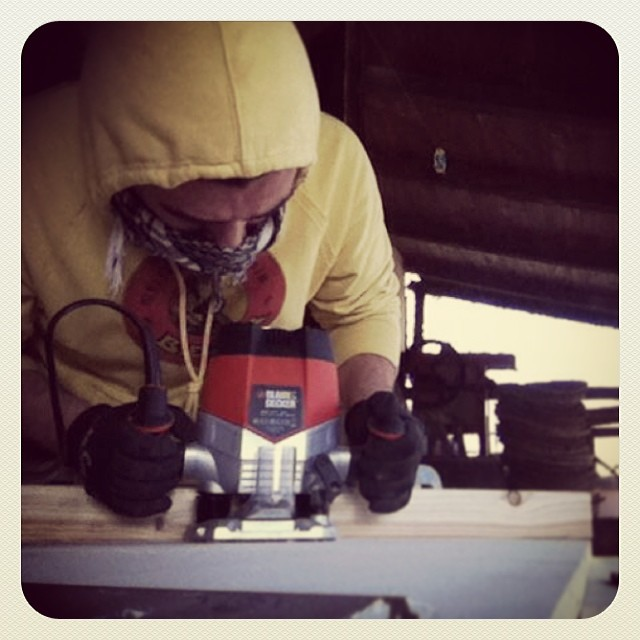
\includegraphics[width=.47\textwidth]{img/image2.jpg}
\caption{Mind Mapping}
\label{gs}
\end{figure}

\begin{equation}
m(x,p,\theta) = (p*x) + ((1-p)*(x\cos\theta)
\label{eq:mid}
\end{equation}

Some predictions of general relativity differ significantly from those of
classical physics, especially concerning the passage of time, the geometry of
space, the motion of bodies in free fall, and the propagation of light.

%--------------------------------------------
%----------------larghezza massima del codice
\begin{lstlisting}
mspan(x,p,rad) = m,s
with{
  m = (p*x)+((1-p)*(x*cos(rad)));
  s = x*(sin(-rad));
};
\end{lstlisting}

Examples of such differences include gravitational time dilation, gravitational
lensing, the gravitational redshift of light, and the gravitational time delay.
The predictions of general relativity in relation to classical physics have been
confirmed in all observations and experiments to date.

\vfill\null

\raggedright
%\bibliographystyle{unsrt}
%\printbibliography

\end{document}

%%%%%%%%%%%%%%%%%%%%%%%%%%%%%%%%%%%%%%%%%%%%%%%%%%%%%%%%%%%%%%%%%%%%%%%%%%%%%%%%
% 2020 GIUSEPPE SILVI ARTICLE TEMPLATE BASED ON
%%%%%%%%%%%%%%%%%%%%%%%%%%%%%%%%%%%%%%%%%%%%%%%%%%%%%%%%%%%%%%%%%%%%%%%%%%%%%%%%
% Journal Article
% LaTeX Template
% Version 1.4 (15/5/16)
% This template has been downloaded from:
% http://www.LaTeXTemplates.com
% Original author:
% Frits Wenneker (http://www.howtotex.com) with extensive modifications by
% Vel (vel@LaTeXTemplates.com)
% License:
% CC BY-NC-SA 3.0 (http://creativecommons.org/licenses/by-nc-sa/3.0/)
%%%%%%%%%%%%%%%%%%%%%%%%%%%%%%%%%%%%%%%%%%%%%%%%%%%%%%%%%%%%%%%%%%%%%%%%%%%%%%%%
